\documentclass{report}
\usepackage[utf8]{inputenc}
\usepackage[swedish]{babel}
\usepackage{url}
\usepackage{hyperref}
\usepackage{graphicx}
\usepackage{float}
\usepackage[hidelinks]{hyperref}

\title{Agenda 2030: Globala mål för hållbar utveckling}
\date{\today}
\author{Johanna Sörbom}

\begin{document}
\maketitle
\newpage
\begin{titlepage}
\section*{Sammanfattning}
\newpage
\tableofcontents
\end{titlepage}
\newpage
\pagenumbering{arabic}
\section{Inledning}
\subsection{Bakgrund}
Under de senaste århundraderna har människan utvecklats i en takt alldrig tidigare skådad.(WWF) Så snabbt att naturen inte har hunnit med.(Sapiens) Detta har bland annat gett upphov till klimatförändringar, utarmade ekosystem, fattigdom och ökande klyftor mellan rika och fattiga länder. (WWF) Idag räcker inte längre med att utveckas, för en bättre framtid krävs utveckling på ett hållbart sätt. Hållbar utveckling är ett stort samtalsämne i dagens samhälle och något som pushas hårt av bland annat FN. Hållbar utveckling definieras som utveckling som tillgodoser dagens behov utan att äventyra kommande generationers möjlighter att tillgodose sina behov.\cite{web2030agenda}
För att driva utvecklingen framåt på ett hållbart sätt för världens u-länder enades FNs medlemsländer år 2000 om Millenniemålen, som behandlar de viktiga punkterna för hållbarhet och utveckling.  Sedan millenniemålen skapades år 2000 har stora framsteg gjort i fattigdomsbekämpning, jämställdhet och utveckling. Men det finns mycket kvar att jobba på. \cite{webEuropeanComission}
Agenda 2030: Globala mål för hållbar utveckling är en ny global utvecklingsagenda framtagen av FN och antagen av världens stats- och regeringschefer som tar vid där millenniemålen slutade år 2015. Denna agenda går djupare in på problemen än vad millenniemålen gjorde. Den fokuserar på hållbar utveckling i alla länder, inte bara u-länder och erkänner arbete mot klimatpåverkan som en grund för att nå en hållbar utveckling. Men kommer denna agenda att lyckas leda världen mot en hållbarare framtid? Världens ledare har uttryckt höga förhoppningar för denna utvecklingsplan som bygger på erfarenhet från millenniemålen. Men ingenting kommer utan en del kritik. 

\subsection{Metod och källkritik}
Denna rapport är sammanställd genom litteraturstudier. De huvudsakliga källorna är FN och Sveriges regeringskansli. 
\newpage 
\section{Resultat}
\subsection{Vad är Agenda 2030: Globala mål för hållbar utveckling och vilka har skrivit på denna agenda?}
Agenda 2030 är en ny global utvecklingsagenda från FN som består av 17 globala mål för hållbar utveckling. \cite{webUNASweden} Agendan\cite{nam2015transforming} är en handlingsplan för människorna, planetens och vårat välstånd. De globala miljömålen tar vid där millenniemålen slutade och består av 169 delmål för en bättre framtid. I september 2015 hos FN i New York skrev samtliga av FNs 193 medlemsstater på Agenda 2030 och de globala målen för hållbar utveckling.\cite{webUNASweden} Målen är universella och gäller både höginkomst- och låginkomstländer \cite{webUNDP}. De Globala målen ska leda världen mot en fredlig och hållbar utveckling till år 2030 och integrerar de tre dimensionerna av hållbar utveckling: social, ekonomisk och miljömässig.  \cite{webUNASweden}\\

 De 17 globala mål som antogs är: 
\begin{enumerate}
\item Utrota fattigdom i alla dess former, överallt.
\item Utrota hunger, uppnå matsäkerhet och förbättrad kost samt främja ett hållbart jordbruk.
\item Säkerställa hälsosamma liv och främja välbefinnande för alla i alla åldrar.
\item Säkerställa inkluderande och rättvis utbildning av god kvalitet och främja livslångt lärande för alla.
\item Uppnå jämställdhet och stärka alla kvinnors och flickors ställning.
\item Säkerställa tillgänglighet och hållbar förvaltning av vatten och sanitet för alla.
\item Säkerställa tillgång till prisvärd, pålitlig, hållbar och modern energi för alla.
\item Främja kontinuerlig, inkluderande och hållbar ekonomisk tillväxt, full och produktiv sysselsättning och anständigt arbete för alla.
\item Bygga motståndskraftig infrastruktur, främja inkluderande och hållbar industrialisering och främja innovation.
\item Minska ojämlikhet inom och mellan länder.
\item Gör städer och boplatser inkluderande, säkra, flexibla och hållbara.
\item Säkerställa hållbara konsumtions- och produktionsmönster.
\item Vidta brådskande åtgärder för att bekämpa klimatförändringarna och dess effekter.
\item Bevara och hållbart nyttja hav, sjöar och marina resurser för hållbar utveckling.
\item Hållbart skogsbruk, stoppa ökenspridning, bromsa och vända markförstöring samt hejda förlusten av biologisk mångfald.
\item Främja fredliga och inkluderande samhällen för hållbar utveckling, ge tillgång till rättssystem för alla och bygga effektiva, ansvarstagande och inkluderande institutioner på alla nivåer.
\item Stärka verktyg för genomförande och vitalisera det globala partnerskapet för hållbar utveckling. \cite{webKTH}
\end{enumerate}

\subsection{Hur ska Agenda 2030 implementeras?} 
Implementering av de Globala målen och framgång kommer att bero på ländernas egna policys, planer och program. De Globala målen ska fungera som en riktlinje för att styra ländernas planer mot det som överenskommits i Agenda 2030. \cite{web2030agenda}
I Sverige har Sida fått i uppdrag av regeringen att utveckla nya innovativa former för utvecklingsfinansiering. \cite{webSIDA}
Nationellt ledda utvecklingsstrategier kommer att kräva mobilisering av resurser och strategier för finansiering. Regeringen, civilsamhället, den privata sektorn och alla andra förväntas samarbeta för att nå de Globala målen. Men även en global gemenskap kommer krävas för att stödja nationella arbeten.\\

\subsection{Vad händer om ett land inte uppnår målen/ inte följer riktlinjerna? Are the Sustainable Development Goals legally binding? Vem är ansvarig för att det här sker?} 
De Globala målen är däremot inte på något sätt bindande. Länder förväntas själva sätta upp en strategi för att nå de 17 globala målen och implementering kommer att hänga på ländernas egna policies och program för hållbar utveckling. Länderna har själva det huvudsakliga ansvaret att följa upp arbetet. Det finns inget som straffar länder som inte gör sin del för att uppnå de Globala målen som undertecknats i Agenda 2030 eftersom agendan är en överenskommelse mellan länder och inte rättsligt bindande. \cite{web2030agenda}\\

\subsection{Hur ska arbetet finansieras?} 
Att förverkliga dessa mål kommer att kräva stora finansiella insatser och  investering i både U- och I-länder. \cite{web2030agenda}
Hur målen ska implementeras och hur finansiella resurser ska mobiliseras ligger till grund för den nya agendan. \url {http://fn.se/vi-gor/vi-utbildar-och-informerar/fn-info/vad-gor-fn-2/fns-arbete-for-utveckling-och-fattigdomsbekampning/agenda-2030-globala-mal-for-hallbar-utveckling} 
Kostnaden beräknas uppgå till trilljoner dollar, \cite{web2030agenda} ca 4500 miljoner USD per år. Detta är trettio gånger mer än det totala årliga biståndet i världen. \url {https://unicef.se/vad-vi-gor/de-nya-globala-utvecklingsmalen} FN:s medlemsländer enades under mötet i New York om ett 100-tal insatser för att finansiera Agenda 2030. Även teknologiöverföring, handel och betydelsen av relevant och bra statistik diskuterades som medel för att uppnå målen. \cite{webUNASweden}
Enligt FN måste resurser mobiliseras från både den kommunala och den privata sektorn, nationellt och internationellt. Det kommer inte att räcka med traditionellt bistånd. Resurserna finns redan i världen men hur investeringar riktas för att stödja hållbar utveckling kommer att spela stor betydelse. Utvecklingshjälp kommer fortfarande att krävas för att hjälpa fattigare länder att nå målen. 
\cite{web2030agenda}
I juli 2015 samlades delegater från hela världen vid FN:s konferens om utvecklingsfinansiering i Addis Abeba. Resultatet blev Addis Ababa Action Agenda, som fastställer hur de Globala målen ska finansieras. \url { http://www.sida.se/Svenska/sa-arbetar-vi/Internationellt-samarbete-/globalamalen/}
I agendan kom länderna överens en mängd åtgärder för att finansiera de Globala målen såsom förbättrad skatteinsamling och åtgärder mot taxsmitning. Samarbete och officiel utvecklingshjälp mellan länder, speciellt U-länder, var en annan överenskommelse. Agendan understryker även hur viktigt det är med privat investering och incitament från regeringen för att leda dessa investeringar mot hållbar utveckling. Ett nytt sätt att finansiera ny teknologi till U-länder var också med i överenskommelsen. Den innefattade även internationellt samarbete för finansiering av områden där investering krävs såsom infrastruktur för energi, transport, vatten och andra områden för att nå de Globala målen.  
\cite{webUNDESA}\\

\subsection{Hur sker uppföljningen och övervakningen?} 
Uppföljning och övervakning av målen och arbetet som görs kommer att ske både på global och nationell nivå. Globalt så kommer målen från den nya agendan att mätas mot ett antal globala indikatorer. Dessa indikatorer togs fram av The Inter-Agency and Expert Group on SDG Indicators (IAEG-SDGs) och slogs igenom i mars 2016. \cite{web2030agenda}
Det finns idag en lista med 232 indikatorer som följs, se bilagor \url {https://unstats.un.org/sdgs/indicators/indicators-list/.}
Regeringar kommer också själva att utveckla nationella indikatorer för att hjälpa till att övervaka framstegen som görs för att nå de 17 målen. Det ska resultera i 2 indikatorer för varje delmål. Uppföljningen av dessa mål kommer att samlas i en rapport för FNs generalsekreterare. De årliga mötena av  “High-level Political Forum on sustainable development” kommer att spela en central roll i utvärderingen av de Globala målen på global nivå. Implementeringsmetoderna kommer att ses igenom för att försäkra att finansiella resurser är mobiliserade på ett effektivt sätt för att nå de Globala målen.  \cite{web2030agenda}\\

\subsection{Vad är skillnaden mellan de globala utvecklingsmålen och millenniemålen? Hur gick det för millenniemålen (jämförelse)? } 
De Globala målen är en fortsättning på millenniemålen som utgick år 2015. Millenniemålen har hjälpt till att väcka uppmärksamhet till mängder av problem i världen. Sedan millenniemålen sattes har världens fattigdom halverats, 90 procent av barn i U-länder får nu grundläggande utbildning och jämställdhet har ökat. Det finns dock mycket kvar att jobba på. \cite{webEuropeanComission}
Sedan 1990 har utsläppen av växthusgaser ökat med nästan 50 procent och de fortsätter öka. Nivån växthusgaser i atmosfären är idag högre än den någonsin varit. (United Nations. 2017. Goal 13: Take urgent action to combat climat change and its impacts. United Nations.
http://www.un.org/sustainabledevelopment/climate-change-2/)
I FNs utvärdering av millenimålen "The Millenium Development Goals report 2015" KÄLLA visas det att alla länder med tydliga mål, strategier och politisk vilja kan göra framsteg mot en bättre värld. Rapporten skriver också att dessa framsteg har varit ojämna och fallit kort i flera områden och inte nått många av världens fattigaste och mest utsatta. I rapporten fastslogs att specialinriktade insatser behövs för att nå världens mest utsatta.  Milleniemålen har även visat hur viktigt det är att följa upp målen med data för att ganomföra målen. Detta är något som de Globala målen bygger vidare på. (The Millenium Development Goals report 2015)

Agenda 2030 bygger på erfarenhet från millenniemålen för att fortsätta jobba mot en hållbar utveckling. \cite{webEuropeanComission}
De Globala målen är mer omfattande än millenniemålen var och adresserar problemen på djupet på ett sätt som ska vara hållbart för alla världens länder. De Globala målen är just globala till skillnad från millenniemålen som endast var riktade i huvudsak mot U-länderna. En viktig del av de Globala målen är att de fokuserar extra mycket på hur de ska implementeras och förverkligas. De nya Globala målen erkänner även att arbete mot klimatförändring är viktigt för hållbar utveckling och bekämpning av fattigdom. \cite{web2030agenda}
Problemen med milleniemålen har varit att framstegen ofta inte når världens mest utsatta människor. De fattigaste och de som lever i konfliktzoner samt de som diskrimineras på grund av kön, ålder, funktionshinder eller etnicitet. Utvecklingen skiljer sig åt mycket mellan länder och trots framsteg finns det  mycket kvar att förbättra. \\

\subsection{Vad är kritiken mot agendan?} 
Trots de höga förhoppningarna från världens ledare som skrivit på Agenda 2030 så har den fått kritik. Thomas Pogge \cite{critique} från Yales Philosophy Department listar upp flera punkter där de globala målen brister: 

\begin{enumerate}
\item De Globala målen främjar en falsk känsla av framgång och gör det lätt för regeringar att ta det långsamt med att förverkliga de mänskliga rättigheter. 
\item De Globala målen misslyckas med att specificera vad en mändklig rättighetsbaserad plikt eller et genuint mål för att utrota fattigdom kräver: en tydlig arbetsfördelning. 
\item Ett fullständigt förverkligande av de mänskliga rättigheterna kräver en omfattande tillbakadragning av internationella och nationella ojämlikheter, vilket de Globala målen inte kräver. 
\end{enumerate} 

SKRIV NÅGOT OM DESSA \\


ICSU och ISSU har satt ihop en rapport där de utvärderar de Globala målen utifrån en vetenskapligt perspektiv. De skriver i sin rapport att de Globala målen är en betydande förbättring av millenniemålen.  De tar upp några av de systematiska hindren för en hållbar utveckling och erbjuder en bättre balans av de tre dimensionerna av hållbar utveckling, social, ekonomisk och miljö. De tar även hänsyn till viktiga faktorer såsom ojämlikhet, ohållbar konsumtion, institutionskapacitet och miljöproblem som millenniemålen utelämnade. Miljömässigt hållbarhet bra något som lades till senare i millenniemålen och spelade inte en lika grundläggande roll som det nu gör i de Globala målen. Millenniemålen fokuserade endast på u-länder och fångade bara till en viss del de tre dimensionerna av hållbarhet. En viktig skillnad med de Globala målen är att de ser att alla världens länder behöver jobba för en hållbar utveckling, även om alla mål inte är lika viktiga för alla länder. Trots alla dessa framsteg finns det förbättringar som skulle kunna göras i Agenda 2030. Enligt ICSU och ISSU utvärdering av delmålen är 49st (29 procent) väl utvecklade, 91st (54 procent) skulle behöva vara mer specifika och 29st (17 procent) kräver betydligt mer arbete. Se figur 1 \ref{fig1}. 
I sin rapport ” Review of targets for the sustainable development goals: The science perspecive” listar de upp fem punkter för förbättring:  

\begin{enumerate}
\item Formulera ett övergripande mål.
\item Utveckla sammanlänkande delmål som är gemensamma för olika mål. 
 \item Formulera en lockande framtidsbild utav utvecklingenscenariet. 
\item Förena och paketera målen och dess interaktioner med varandra.
\item Specificera delmålen.
\end{enumerate} 
KÄLLA PDF SDG\\

\begin{figure}[h] \label{fig1}
\label{improvments}
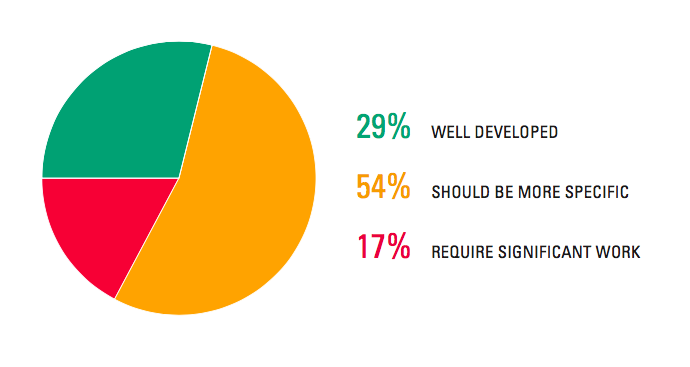
\includegraphics[width=\linewidth]{improvments.png}
\caption{De Globala målen KÄLLA} 
\end{figure}

Förbättringsmöjlighet 1 syftar på att de Globala skulle kunna gynnas av ett övergripande mål som binder samman de 17 målen och beskriver hur dessa mål ska komma till nytta för världen och dess invånare. Även viktiga avvägningar och komplementeringar som rör målen skulle kunna gynnas av att specificeras i ett uppföljningsdokument. ICSU och ISSU har som exempel “a prosperous, high quality of life that is equitably shared and sustainable”. Detta övergripande mål skulle också kunna hjälpa till att göra agendan med tillgänglig och förståelig för en större mängd människor. (Costanza R., 2014. a theory of socio-ecological system change. journal of BioEconomics, 16:39-44.)\\

Med förbättringsmöjlighet 2 menas att 

(weitz N., m. Nilsson and m. Davis, 2014. a nexus approach to the post-2015 agenda: formulating integrated water, energy and food SDGs. SaIS Review of International affairs, 34:37-50.)


 Det nuvarande ramverket för de Globala målen identifierar inte heller de olika sociala grupper som kommer att behöva arbeta för att uppnå målen tilsammans med regeringar. 





Är det tillräckligt tydliga delmål, hur målen ska uppnås?
Har någon utveckling skett sedan Agenda 2030 skapades?



\newpage
\section{Diskussion}
Att de Globala målen inte är bindande kan ses som både en fördel och en nackdel. Eftersom agedan är en överenskommelse mellan länder och inte rättsligt bindande skapar det en möjlighet för länder att fly från sina förpliktelser. Men det skapar även möjlighet för länder att anta en mer ambitiös agenda om så önskas. \cite{critique} Efetrsom länder har olika förutsättningar att uppnå målen kan det krävas olika mål för olika länder. Länder som kan göra mer borde göra mer och hjälpa de länder som behöver financiellt stöd för att nå de satta målen. Globalt sammarbete är något som understryks i agendan och som förhoppningsvis faktiskt kan ske. Detta kräver att länder kan se utöver sina egna gränser eftersom detta är ett världsomfattande problem. Precis som när milleniemålen skapades så har Fn:s alla medlemsstater skrivit under agendan. Detta är mycket possitivt då det ligger i allas intresse att jobba mot en hållbar utveckling. Eftersom de Globala målen har erkänt arbete mot klimatpåverkan som en grund för att uppnå målen kan det ses som ett framsteg att alla länder har skrivit på agendan. Tidigare klimatmöten såsom COP15 har let till urvattnade förslag då länder inte kunnat komma överens. 


\newpage
\section{Slutsats}
Trots en del repetition av millenniemålen och många svagt formulerade mål är Agenda 2030: Globala mål för hållbar utveckling en stor framgång. De har utvecklats med lärdomar som millenniemålen gav i åtanke och har resulterat i starkare och bättre Globala mål. 
\bibliographystyle{plain}
\bibliography{references} 



\end{document}
